\section{Segunda mitad del siglo XX}
 
Hasta ahora no hemos mencionado ningún ejemplo sobre el uso de la Computación en las investigaciones biológicas.
Esto tiene una explicación muy simple, durante la primera mitad del siglo XX el acceso a medios computacionales era escaso.
Como referencia, fue en 1946 que se terminó de construir la primera computadora electrónica de uso general, la ENIAC.
En estas etapas iniciales solo las instituciones más grandes (como los gobiernos y los ejércitos) tenían acceso a estas máquinas.
Pero a finales de los 50's esta tendencia fue cambiando, ya comenzaba a ser común para algunas universidades disponer de estos medios.
 
\begin{figure}[tb]
   \centering
   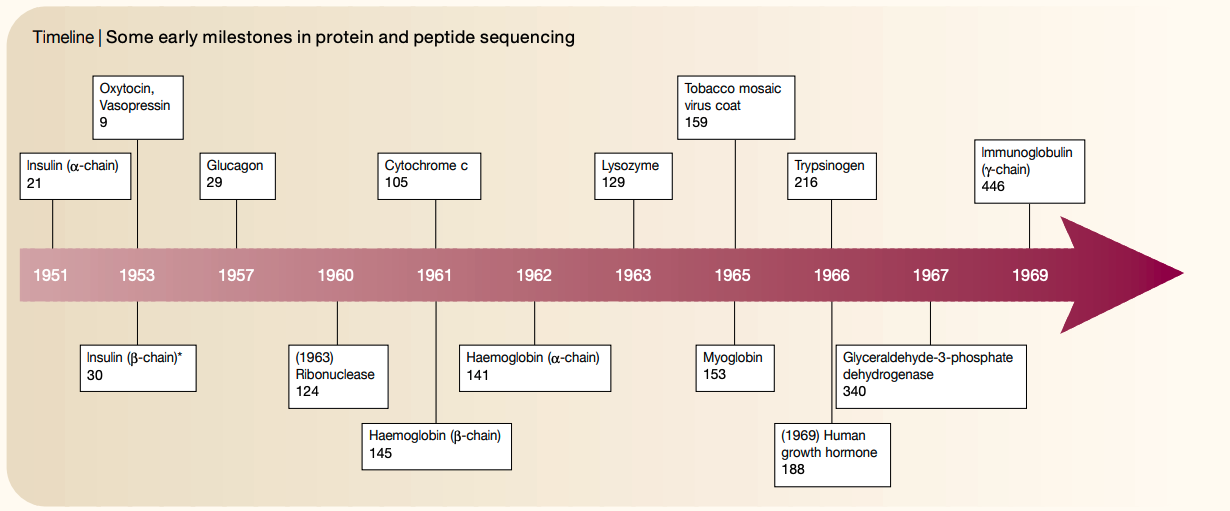
\includegraphics[width=1.0\columnwidth]{images/Protain_seq_milestones.png}
   \caption{
       (\textit{Figura en inglés})
       Momentos claves iniciales en el proceso de secuenciación de proteínas.
       Los números debajo de los nombres de las proteínas indican el número de aminoácidos de su secuencia (ej: Glucagón: 29).
       Fuente \cite{hagenOriginsBioinformatics2000}}
   \label{fig:Protain_seq_milestones}
\end{figure}
 
Mientras tanto, el primer enunciado formal del dogma central de la Biología Molecular fue expuesto por el propio Francis Crick durante una conferencia en 1957 \cite{cobb60YearsAgo2017}.
En este, las secuencias de ADN juegan el papel central como punto de partida del flujo de la información que caracteriza el desarrollo de los organismos.
A pesar de esto, por limitaciones experimentales de la época, son las secuencias proteicas las que son más accessibles.
Luego de que las primeras proteínas fueran resueltas ``a mano'', desde principios de los 60's se comienza a automatizar el proceso.
Proteínas cada vez más ``largas'' se secuenciaron en cada vez menos tiempo (figura \ref{fig:Protain_seq_milestones}).
A finales de los 60's, Pehr Edman diseñó el \textit{sequenator} \cite{edmanProteinSequenator1967}, un equipo completamente automático.
Cada vez más laboratorios se aventuraban a secuenciar proteínas de interés y así surgieron los primeros repositorios de secuencias \cite{hagenOriginsBioinformatics2000}.
 
\begin{figure}[h]
   \centering
   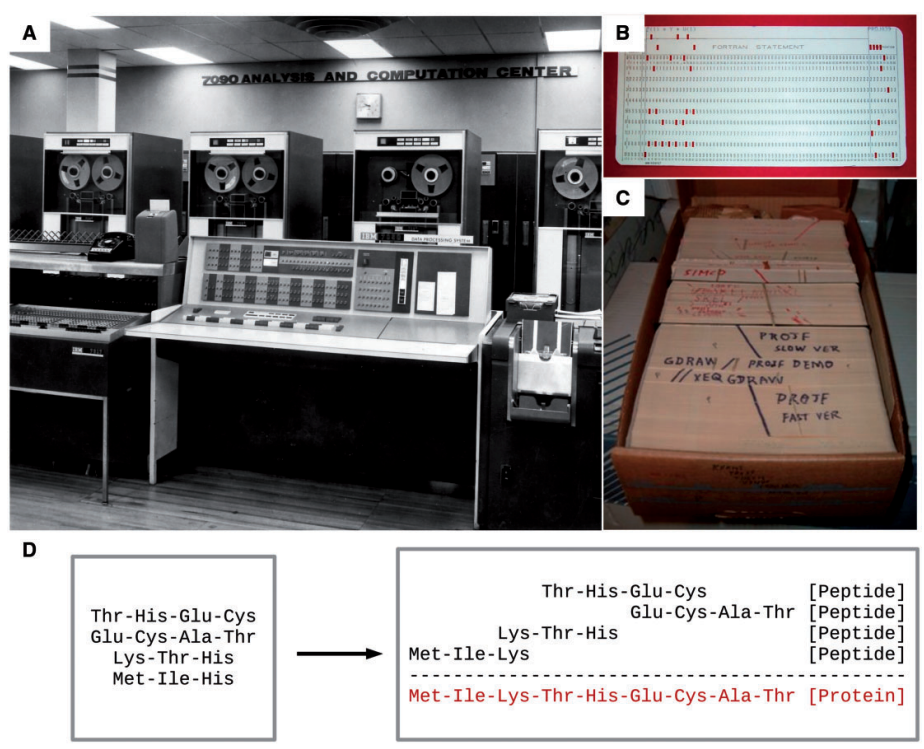
\includegraphics[width=0.7\columnwidth]{images/COMPROTEIN.png}
   \caption{
       Lo que es considerado como uno de los primeros sistemas bioinformáticos.
       \textbf{Panel A}: una computadora de la época (1962).
       \textbf{Panel B}: una tarjeta perforada (un medio de almacenamiento digital ``antiguo'').
       \textbf{Panel C}: conjunto de miles de tarjetas perforadas que contienen el programa ensamblador.
       \textbf{Panel D}: representación del proceso de ensamblaje de la secuencia completa a partir de los fragmentos secuenciados.
       Fuente \cite{gauthierBriefHistoryBioinformatics2019}}
   \label{fig:COMPROTEIN}
\end{figure}
 
% 5
El uso de las computadoras durante el proceso de secuenciación fue imprescindible desde bien temprano (figura \ref{fig:COMPROTEIN}) \cite{dayhoffAComputerProgram1962}.
El problema principal radicaba en que los métodos bioquímicos de la época solo podían resolver en cada corrida secuencias de tamaño limitado.
Por ello, para secuenciar proteínas de mayor tamaño, estas eran divididas en fragmentos manejables que se procesaban individualmente.
Luego, la secuencia completa de la proteína era reconstruida aprovechando secciones redundantes entre los fragmentos adyacentes.
La complejidad del proceso reconstructivo aumenta considerablemente con el tamaño de las proteínas y la cantidad de fragmentos en cuestión, por lo que rápidamente se hace impráctico realizarlo manualmente.

%  5
Los años 50's y 60's son etapas muy tempranas en el desarrollo de la Computación.
El hecho de que ya desde esta época la Biología asimilara su uso pone de manifiesto un patrón universal en la ciencia.
No existen herramientas únicas de un campo o disciplina, o herramientas que no sean de su interés.
Esas ideas son, en el mejor de los casos, solo una ilusión temporal.
Lo que existen son problemas, cuestiones que se quieren resolver.
El cómo atacarlos cambia dependiendo de qué recursos estén disponibles.
Seguramente Albert Eistein no estudió programación en la universidad (las computadoras no eran muy populares por esa época), sin embargo, pero al tiempo de su muerte en 1955, los físicos ya habían incorporado esta a su caja de herramientas.

% 5
Sin embargo, el impacto del uso de la Computación en las investigaciones biológicas solo comenzaba.
La acumulación de secuencias de proteínas potenció el desarrollo de nuevas ramas dentro de esta ciencia.
Una de las más tempranas fue el campo de la Evolución Molecular.
El dogma central tiene consecuencias muy interesantes.
Primero, al ser el ADN el principal portador de la información genética, la evolución puede ser vista como la acumulación de cambios en dicha secuencia y su posterior discriminación por seleción natural.
De esta manera, una comparación de secuencias de diferentes especies debería arrojar luz sobre su pasado evolutivo.
Segundo, que se puede aprender sobre las secuencias de ADN partiendo del estudio de las secuencias de las proteínas.
Así, los estudios evolutivos también se podían llevar a cabo empleando las secuencias de estas últimas.
 
\begin{figure}[h]
   \centering
   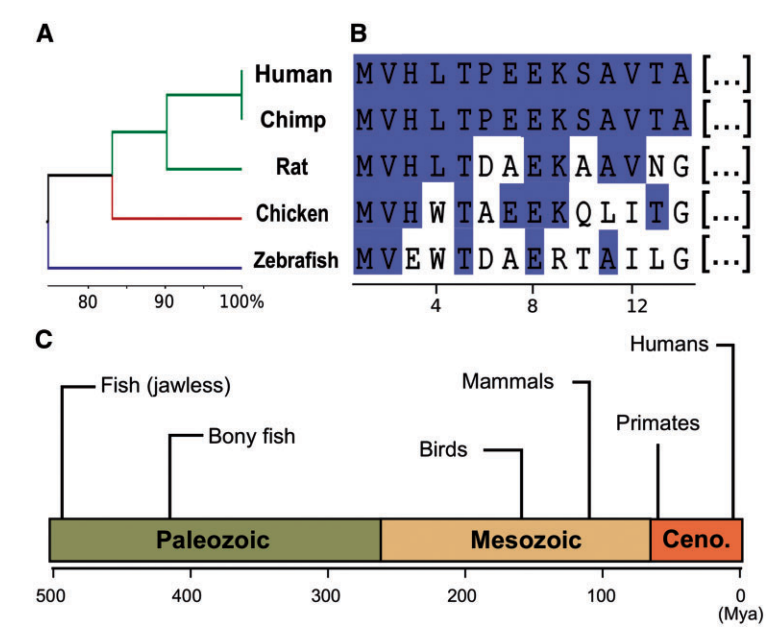
\includegraphics[width=0.7\columnwidth]{images/evolution.png}
   \caption{
       (\textit{Figura en inglés})
       \textbf{Panel A y B}: el árbol filogenético (izquierda) y un fragmento de la comparación (derecha) entre las secuencias de hemoglobina que se emplearon en su elaboración (cada letra representa un aminoácido).
       \textbf{Panel C}: cronología de los fósiles más antiguos encontrados de las especies/grupos estudiados (\textit{Mya} Millones de años).
       Fuente \cite{gauthierBriefHistoryBioinformatics2019}}
   \label{fig:evolution}
\end{figure}

% 5
La hipótesis era simple.
Si dos especies divergieron recientemente en la historia evolutiva, las secuencias de proteínas comunes a ambas (denominadas homólogas) deberían ser similares.
Por el contrario, si las especies están muy poco emparentadas, esta similitud se espera sea menor.
De esa forma, ordenando un grupo de especies con respecto a la ``similitud'' entre sus secuencias homólogas, se podría construir su árbol filogenético.
Por ejemplo, si se compara la secuencia de la hemoglobina humana con la del chimpancé se aprecian menos diferencias que entre un humano y un ratón.
Los árboles filogenéticos obtenidos de esta forma fueron luego comparados,  con muy buenos resultados, con los obtenidos mediante los métodos tradicionales, como el registro fósil (figura \ref{fig:evolution}) \cite{fitchConstructionPhylogeneticTrees1967}.

% 5
Una vez más, la Computación fue clave en estas investigaciones.
Mientras más secuencias de más especies se acumulaban, realizar el alineamiento necesario para determinar su similitud se hacía demandante, incluso, para las computadoras más avanzadas;
sobre todo si las especies estudiadas estaban muy poco emparentadas y las diferencias entre las secuencias eran pronunciadas o implicaban adiciones o eliminaciones.
Como referencia, comparar solo $10$ secuencias de $100$ aminoácidos de extensión cada una tomaba como promedio $10^{18}$ operaciones \cite{wangComplexityMultipleSequence1994}.
Estas investigaciones no solo estaban en la vanguardia de la Biología, sino también de la Computación.
Como veremos a continuación esta tendencia llega hasta hoy día.
La relación entre ambas ciencias siempre ha sido de beneficio mutuo y con una clara inclinación a profundizarse.
